% AUTO-GENERATED by code/ch6_figs.py
\begin{tabular}{@{}r@{\hspace{8pt}}c@{\hspace{8pt}}l@{}}
input $\bm{x}$ & $\vcenter{\hbox{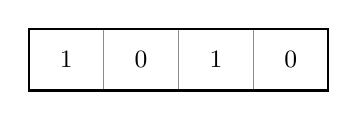
\begin{tikzpicture} \draw[black!45, fill=white] (0.000,0.000) rectangle (0.950,-0.779); \node[font=\small, text=black] at (0.475,-0.389) {$1$}; \draw[black!45, fill=white] (0.950,0.000) rectangle (1.900,-0.779); \node[font=\small, text=black] at (1.425,-0.389) {$0$}; \draw[black!45, fill=white] (1.900,0.000) rectangle (2.850,-0.779); \node[font=\small, text=black] at (2.375,-0.389) {$1$}; \draw[black!45, fill=white] (2.850,0.000) rectangle (3.800,-0.779); \node[font=\small, text=black] at (3.325,-0.389) {$0$}; \draw[line width=0.9pt] (0.000,0.000) rectangle (3.800,-0.779); \end{tikzpicture}}}$ & \tok{waste}\\[3pt]
minus the mean $\mu$ & $\vcenter{\hbox{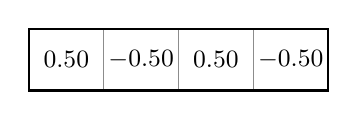
\begin{tikzpicture} \draw[black!45, fill=white] (0.000,0.000) rectangle (0.950,-0.779); \node[font=\small, text=black] at (0.475,-0.389) {$0.50$}; \draw[black!45, fill=white] (0.950,0.000) rectangle (1.900,-0.779); \node[font=\small, text=black] at (1.425,-0.389) {$-0.50$}; \draw[black!45, fill=white] (1.900,0.000) rectangle (2.850,-0.779); \node[font=\small, text=black] at (2.375,-0.389) {$0.50$}; \draw[black!45, fill=white] (2.850,0.000) rectangle (3.800,-0.779); \node[font=\small, text=black] at (3.325,-0.389) {$-0.50$}; \draw[line width=0.9pt] (0.000,0.000) rectangle (3.800,-0.779); \end{tikzpicture}}}$ & $\mu = 0.500$, subtracted from every entry\\[3pt]
divide by $\sigma$ & $\vcenter{\hbox{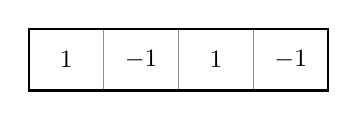
\begin{tikzpicture} \draw[black!45, fill=white] (0.000,0.000) rectangle (0.950,-0.779); \node[font=\small, text=black] at (0.475,-0.389) {$1$}; \draw[black!45, fill=white] (0.950,0.000) rectangle (1.900,-0.779); \node[font=\small, text=black] at (1.425,-0.389) {$-1$}; \draw[black!45, fill=white] (1.900,0.000) rectangle (2.850,-0.779); \node[font=\small, text=black] at (2.375,-0.389) {$1$}; \draw[black!45, fill=white] (2.850,0.000) rectangle (3.800,-0.779); \node[font=\small, text=black] at (3.325,-0.389) {$-1$}; \draw[line width=0.9pt] (0.000,0.000) rectangle (3.800,-0.779); \end{tikzpicture}}}$ & $\sigma = 0.500$, the spread of the line above\\[3pt]
times gain $\bm{g}$ & $\vcenter{\hbox{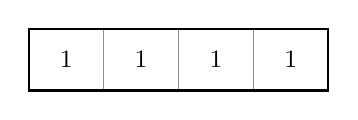
\begin{tikzpicture} \draw[black!45, fill=white] (0.000,0.000) rectangle (0.950,-0.779); \node[font=\small, text=black] at (0.475,-0.389) {$1$}; \draw[black!45, fill=white] (0.950,0.000) rectangle (1.900,-0.779); \node[font=\small, text=black] at (1.425,-0.389) {$1$}; \draw[black!45, fill=white] (1.900,0.000) rectangle (2.850,-0.779); \node[font=\small, text=black] at (2.375,-0.389) {$1$}; \draw[black!45, fill=white] (2.850,0.000) rectangle (3.800,-0.779); \node[font=\small, text=black] at (3.325,-0.389) {$1$}; \draw[line width=0.9pt] (0.000,0.000) rectangle (3.800,-0.779); \end{tikzpicture}}}$ & all 1 in the toy\\[3pt]
output & $\vcenter{\hbox{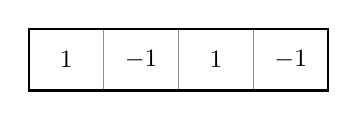
\begin{tikzpicture} \draw[black!45, fill=white] (0.000,0.000) rectangle (0.950,-0.779); \node[font=\small, text=black] at (0.475,-0.389) {$1$}; \draw[black!45, fill=white] (0.950,0.000) rectangle (1.900,-0.779); \node[font=\small, text=black] at (1.425,-0.389) {$-1$}; \draw[black!45, fill=white] (1.900,0.000) rectangle (2.850,-0.779); \node[font=\small, text=black] at (2.375,-0.389) {$1$}; \draw[black!45, fill=white] (2.850,0.000) rectangle (3.800,-0.779); \node[font=\small, text=black] at (3.325,-0.389) {$-1$}; \draw[line width=0.9pt] (0.000,0.000) rectangle (3.800,-0.779); \end{tikzpicture}}}$ & entries add to 0; length $= 2.000$\\[3pt]
\end{tabular}
